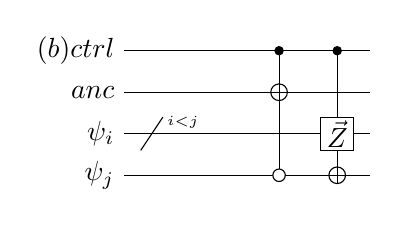
\begin{tikzpicture}[scale=1.000000,x=1pt,y=1pt]
\filldraw[color=white] (0.000000, -7.500000) rectangle (89.000000, 52.500000);
% Drawing wires
% Line 1: ctrl W \text{(b) }ctrl
\draw[color=black] (0.000000,45.000000) -- (89.000000,45.000000);
\draw[color=black] (0.000000,45.000000) node[left] {$\text{(b) }ctrl$};
% Line 2: anc W anc
\draw[color=black] (0.000000,30.000000) -- (89.000000,30.000000);
\draw[color=black] (0.000000,30.000000) node[left] {$anc$};
% Line 3: i W \psi_i
\draw[color=black] (0.000000,15.000000) -- (89.000000,15.000000);
\draw[color=black] (0.000000,15.000000) node[left] {$\psi_i$};
% Line 4: j W \psi_j
\draw[color=black] (0.000000,0.000000) -- (89.000000,0.000000);
\draw[color=black] (0.000000,0.000000) node[left] {$\psi_j$};
% Done with wires; drawing gates
% Line 6: i / ^{i<j}
\draw (6.000000, 9.000000) -- (14.000000, 21.000000);
\draw (12.000000, 18.000000) node[right] {$\scriptstyle{^{i<j}}$};
% Line 7: ctrl anc i j LABEL
% Line 8: ctrl -j +anc
\draw (56.000000,45.000000) -- (56.000000,0.000000);
\filldraw (56.000000, 45.000000) circle(1.500000pt);
\draw[fill=white] (56.000000, 0.000000) circle(2.250000pt);
\begin{scope}
\draw[fill=white] (56.000000, 30.000000) circle(3.000000pt);
\clip (56.000000, 30.000000) circle(3.000000pt);
\draw (53.000000, 30.000000) -- (59.000000, 30.000000);
\draw (56.000000, 27.000000) -- (56.000000, 33.000000);
\end{scope}
% Line 10: i G $\vec{Z}$ ctrl +j
\draw (77.000000,45.000000) -- (77.000000,0.000000);
\begin{scope}
\draw[fill=white] (77.000000, 15.000000) +(-45.000000:8.485281pt and 8.485281pt) -- +(45.000000:8.485281pt and 8.485281pt) -- +(135.000000:8.485281pt and 8.485281pt) -- +(225.000000:8.485281pt and 8.485281pt) -- cycle;
\clip (77.000000, 15.000000) +(-45.000000:8.485281pt and 8.485281pt) -- +(45.000000:8.485281pt and 8.485281pt) -- +(135.000000:8.485281pt and 8.485281pt) -- +(225.000000:8.485281pt and 8.485281pt) -- cycle;
\draw (77.000000, 15.000000) node {$\vec{Z}$};
\end{scope}
\filldraw (77.000000, 45.000000) circle(1.500000pt);
\begin{scope}
\draw[fill=white] (77.000000, 0.000000) circle(3.000000pt);
\clip (77.000000, 0.000000) circle(3.000000pt);
\draw (74.000000, 0.000000) -- (80.000000, 0.000000);
\draw (77.000000, -3.000000) -- (77.000000, 3.000000);
\end{scope}
% Done with gates; drawing ending labels
% Done with ending labels; drawing cut lines and comments
% Done with comments
\end{tikzpicture}
